\documentclass[a4paper, 12pt]{article}%тип документа

%отступы
\usepackage[left=2cm,right=2cm,top=2cm,bottom=3cm,bindingoffset=0cm]{geometry}

%Русский язык
\usepackage[T2A]{fontenc} %кодировка
\usepackage[utf8]{inputenc} %кодировка исходного кода
\usepackage[english,russian]{babel} %локализация и переносы

%Вставка картинок
\usepackage{wrapfig}
\usepackage{graphicx}
\graphicspath{{pictures/}}
\DeclareGraphicsExtensions{.pdf,.png,.jpg}

%оглавление
\usepackage{titlesec}
\titlespacing{\chapter}{0pt}{-30pt}{12pt}
\titlespacing{\section}{\parindent}{5mm}{5mm}
\titlespacing{\subsection}{\parindent}{5mm}{5mm}
\usepackage{setspace}

%Графики
\usepackage{multirow}
\usepackage{pgfplots}
\pgfplotsset{compat=1.9}

%Математика
\usepackage{amsmath, amsfonts, amssymb, amsthm, mathtools}

%Заголовок
\author{Валеев Рауф Раушанович \\
группа 825}
\title{\textbf{Работа 4.3.3\\Исследование разрешающей способности микроскопа методом Аббе}}
\newtheorem{task	}{Задача}
\begin{document}
\maketitle
\section{Теория}
\textit{Разрешающей способностью оптического прибора} называют минимальное расстояние $l_{\min}$ между двумя точками в пространстве предметов, изображения которых разрешаются по методу Релея. 

Пусть предмет на $L = 25$ см и диаметр зрачка глаза --- $d_0 = 5$ мм. Тогда, согласно \textit{критерию Релея} 
\[\dfrac{l_{\min}}{L} = \dfrac{\lambda}{d_0} \Rightarrow l_{\min} \approx 50 \lambda\]

Подобное можно рассчитать для лупы и прочих оптических приборов.

\begin{figure}[h]
\begin{center}
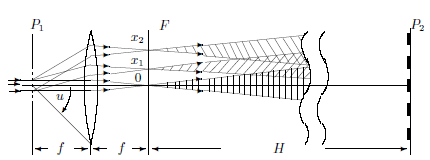
\includegraphics[width = 0.7\textwidth]{1.png}
\caption{Образование изображения в объективе микроскопа.}
\end{center}
\end{figure}

Если наблюдения ведутся при внешнем освещении, то когерентные волны рассеивают различные точки предмета. Схема образования изображения представлена на рис. 1.

\subsection*{Подход Аббе к нахождению разрешающей способности микроскопа}
Разобьем путь лучей от предмета к изображению на 2 этапа:
\begin{enumerate}
\item Картина, возникающая в задней фокальной плоскости $F$ --- \textit{первичное изображение}. 
\item Первичное изображение --- источник волн $\Rightarrow$. Из этих волн возникает \textit{вторичное изображение}.
\end{enumerate}

Легко видеть, что первичное изображение представляет собой картину дифракции Фраунгофера. 

\begin{figure}[h]
\begin{center}
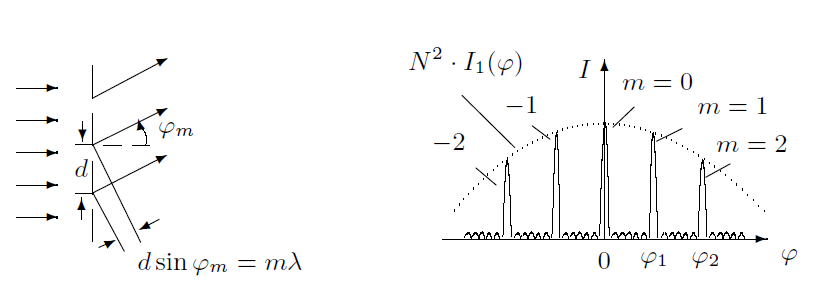
\includegraphics[width = 0.8\textwidth]{2.png}
\caption{Спектр амплитудной решетки}
\end{center}
\end{figure}
При дифракции Фраунгофера на решетке периода $d$ направления $\varphi_m$ максимальной интенсивности определяются из условия 
\begin{equation}
d \sin \varphi_m = m \lambda
\end{equation}

Из рис. 2 легко видеть, что у различных максимумов разные интенсивности.
В итоге у нас излучение точечных источников на равном расстоянии, отсюда интерференция. 

При таком рассмотрении, из того, что линза конечна следует, что есть дифракционные искажения, так как проходят только те волны, для которых верно 
\begin{equation}
\varphi_m < u
\end{equation}

где $u$ --- \textit{апертурный угол} (см. рис. 1).

\begin{wrapfigure}{r}{0.3\textwidth}
  \begin{center}
    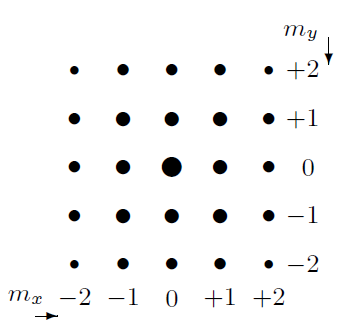
\includegraphics[width = 0.25\textwidth]{3.png}
  \end{center}
  \caption{Дифракция Фраунгофера на двумерной решетке}
\end{wrapfigure}

Если приоткрыть диафрагму и пустить нулевой и 1 из первых максимумов, то получим периодическую картинку, рассчитаем период. $x_1$ между нулевым и первыми максимумами ---
\begin{equation}
x_1 \approx f \varphi_1 = f \lambda/d
\end{equation} 

Ширина интерференционных полос:
\begin{equation}
l = \lambda/\omega
\end{equation} 

где $\omega = x_1/H$ --- угол схождения интерферирующих лучей в точке наблюдения, а $H$ --- расстояние между $F$ и $P_2$. Таким образом, 
\begin{equation}
l \approx \lambda H/x_1 = H d/f
\end{equation}

\begin{equation}
d' \approx \dfrac{H + f}{f} d
\end{equation}

Условие разрешения решетки с периодом $d$:
\begin{equation}
\sin u \geqslant \lambda/d \Rightarrow 
\end{equation}
  
\begin{equation}
d \geqslant \dfrac{\lambda}{\sin u} \approx \dfrac{\lambda}{D/2f}
\end{equation}
Если есть не только 0 максимум, то 
\begin{equation}
d \geqslant \dfrac{\lambda}{2 \sin u}
\end{equation}

У нас решетка двумерная, поэтому мы можем записать все тоже самое в двух осях и получить картину как на рис. 3.
\section{Установка}

\begin{figure}[h]
\begin{center}
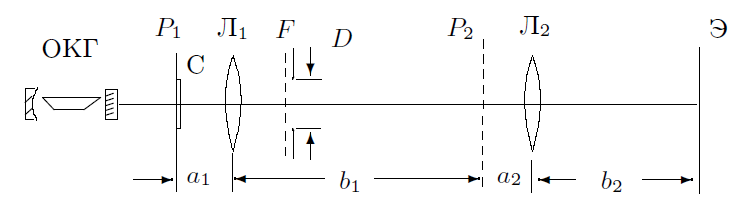
\includegraphics[width = 0.8\textwidth]{4.png}
\caption{Схема установки}
\end{center}
\end{figure}

\section{Ход работы}
Везде ниже мы работаем с зеленым светом у которого длина волны 
\[\lambda = 532 \text{нм}\]
\subsection{Определения периода решеток по спектру}
\begin{enumerate}
\item Соберем установку. 
\item Измерим расстояние между удаленными друг от друга максимумами и число промежутков между ними.
\[l = \dfrac{\Delta l}{n}\]
\item Используя формулу $(1)$ мы можем найти $d$. Причем мы считаем, что 
$\sin \varphi_m \approx \varphi_m$, поскольку у нас маленький угол, а отсюда $\varphi_m = \frac{m \cdot l}{H}$. 
\item Измерим $H$ --- расстояние от сетки до экрана. 

В ниже приведенной таблице погрешности для $\Delta l$ и $H$ берется как половина цены деления линейки, для $l$ считается по формуле
\[\delta(l) = \dfrac{\Delta l}{n}\]
Для $\varphi_1$ считается по формуле
\[\delta(\varphi_1) = \varphi_1 \cdot \sqrt{\left(\dfrac{\delta(l)}{l}\right)^2 + \left( \dfrac{\delta(H)}{H}\right)^2}\]
Из формулы $(1)$ получаем как $d$, так и формулу для ее погрешности, а именно 
\[\delta(d) = d \cdot \left|\dfrac{\delta(\varphi_1)}{\varphi_1}\right|\]
\begin{table}[h!]
\begin{center}
\begin{tabular}{|c|c|c|c|c|c|c|c|c|c|c|c|}
\hline
\multicolumn{10}{|c|}{для горизонтальной составляющей решетки}                                                                                                                                                                                                                                                                                                                                                                          & \begin{tabular}[c]{@{}c@{}}$H$, \\ см\end{tabular} & \begin{tabular}[c]{@{}c@{}}$\delta(H)$, \\ см\end{tabular} \\ \hline
$N_{\text{решетки}}$ & \begin{tabular}[c]{@{}c@{}}$\Delta l$, \\ мм\end{tabular} & \begin{tabular}[c]{@{}c@{}}$\delta(\Delta l)$, \\ мм\end{tabular} & $n$ & \begin{tabular}[c]{@{}c@{}}$l$, \\ мм\end{tabular} & \begin{tabular}[c]{@{}c@{}}$\delta(l)$, \\ мм\end{tabular} & $\varphi_1 \cdot 10^3$ & $\delta( \phi_1) \cdot 10^3$ & \begin{tabular}[c]{@{}c@{}}$d$, \\ мкм\end{tabular} & \begin{tabular}[c]{@{}c@{}}$\delta(d)$, \\ мкм\end{tabular} & \multirow{12}{*}{160,00}                           & \multirow{12}{*}{0,05}                                     \\ \cline{1-10}
1   & 145,0                                                     & 0,5                                                               & 4   & 36,25                                              & 0,13                                                       & 22,66                  & 0,08                         & 23,48                                               & 0,08                                                        &                                                    &                                                            \\ \cline{1-10}
2   & 97,0                                                      & 0,5                                                               & 4   & 24,25                                              & 0,13                                                       & 15,16                  & 0,08                         & 35,10                                               & 0,18                                                        &                                                    &                                                            \\ \cline{1-10}
3   & 97,0                                                      & 0,5                                                               & 8   & 12,13                                              & 0,06                                                       & 7,58                   & 0,04                         & 70,2                                                & 0,4                                                         &                                                    &                                                            \\ \cline{1-10}
4   & 63,0                                                      & 0,5                                                               & 10  & 6,30                                               & 0,05                                                       & 3,94                   & 0,03                         & 135,1                                               & 1,1                                                         &                                                    &                                                            \\ \cline{1-10}
5   & 65,0                                                      & 0,5                                                               & 14  & 4,64                                               & 0,04                                                       & 2,90                   & 0,02                         & 183,3                                               & 1,4                                                         &                                                    &                                                            \\ \cline{1-10}
\multicolumn{10}{|c|}{для вертикальной составляющей решетки}                                                                                                                                                                                                                                                                                                                                                                            &                                                    &                                                            \\ \cline{1-10}
1   & 145,0                                                     & 0,5                                                               & 4   & 36,25                                              & 0,13                                                       & 22,66                  & 0,08                         & 23,48                                               & 0,08                                                        &                                                    &                                                            \\ \cline{1-10}
2   & 97,0                                                      & 0,5                                                               & 4   & 24,25                                              & 0,13                                                       & 15,16                  & 0,08                         & 35,10                                               & 0,18                                                        &                                                    &                                                            \\ \cline{1-10}
3   & 97,0                                                      & 0,5                                                               & 8   & 12,13                                              & 0,06                                                       & 7,58                   & 0,04                         & 70,2                                                & 0,4                                                         &                                                    &                                                            \\ \cline{1-10}
4   & 63,0                                                      & 0,5                                                               & 10  & 6,30                                               & 0,05                                                       & 3,94                   & 0,03                         & 135,1                                               & 1,1                                                         &                                                    &                                                            \\ \cline{1-10}
5   & 65,0                                                      & 0,5                                                               & 14  & 4,64                                               & 0,04                                                       & 2,90                   & 0,02                         & 183,3                                               & 1,4                                                         &                                                    &                                                            \\ \hline
\end{tabular}
\caption{Данные об измерении горизонтального и вертикального периода решетки}
\end{center}
\end{table}
\item Из таблицы видно, что у нас решетка одинакова во всех направлениях (период решетки вертикальный и горизонтальный совпадают).
\end{enumerate}
\subsection{Определения периода решетки по микроскопу}
\begin{enumerate}
\item Соберем и настроим установку как показано на рис. 4.
\item Определим $a_1, b_1, a_2, b_2$ (рис.4), измерим периоды сеток на экране. Учтем так же факт, что $a_2 \approx f_2$. Запишем все значения в таблицу. 

Все погрешности берутся как половина цены деления линейки. Поскольку $f_1$ и $f_2$ (а соответственно и $a_2$) даны сразу, то их можно считать без погрешностей.

\begin{table}[h!]
\begin{center}
\begin{tabular}{|c|c|c|}
\hline
Велечина  & Значение & Погрешность \\ \hline
$a_1$, мм & 130      & 0,5         \\ \hline
$a_2$, мм & 32       & -           \\ \hline
$b_1$, мм & 508      & 0,5         \\ \hline
$b_2$, мм & 670      & 0,5         \\ \hline
$f_1$, мм & 110      & -           \\ \hline
$f_2$, мм & 32       & -           \\ \hline
\end{tabular}
\caption{Геометрические параметры установки, подобранные в ходе эксперимента}
\end{center}
\end{table}
\item В итоге, в получившемся микроскопе у нас получается увеличение в $(b_1b_2)/(a_1a_2)$ раз, то есть измерив период сетки и поделив на данный коэффициент, мы получим период сетки истинный.  То есть, в обозначениях, используемых в таблице $\Delta L$ --- $n$ увеличенных периодов, соответственно увеличенный период --- $L$, а то, что нам нужно найти 
\[d = \dfrac{a_1 a_2}{b_1 b_2} \cdot L\]

\begin{table}[h!]
\begin{center}
\begin{tabular}{|c|c|c|c|c|c|c|c|}
\hline
$N_{\text{решетки}}$ & $\Delta L$, мм & $\delta(\Delta(L))$, мм & $n$ & $L$, мм & $\delta(L)$, мм & $d$, мкм & $\delta(d)$, мкм \\ \hline
1                    & 10,0           & 0,5                     & 8   & 1,25    & 0,06            & 23,7     & 1,2              \\ \hline
2                    & 30,0           & 0,5                     & 16  & 1,88    & 0,03            & 35,5     & 0,6              \\ \hline
3                    & 40,0           & 0,5                     & 11  & 3,64    & 0,05            & 68,8     & 0,9              \\ \hline
4                    & 35,0           & 0,5                     & 5   & 7,00    & 0,10            & 133      & 2                \\ \hline
5                    & 49,0           & 0,5                     & 5   & 9,80    & 0,10            & 186      & 2                \\ \hline
\end{tabular}
\caption{Таблица периода решеток с промежуточными величинами}
\end{center}
\end{table}
\end{enumerate}

Погрешности в таблице взялись: для $\Delta L$ как половина цены деления линейки, для $L$ по формуле $\delta(L) = \frac{\delta(\Delta L)}{\Delta L}$ и для $d$, как видно из формулы
\[\delta(d) = d \cdot \sqrt{\left( \dfrac{\delta(a_1)}{a_1}\right)^2+\left( \dfrac{\delta(a_2)}{a_2}\right)^2+\left( \dfrac{\delta(b_1)}{b_1}\right)^2 + \left( \dfrac{\delta(b_2)}{b_2}\right)^2 + \left( \dfrac{\delta(L)}{L}\right)^2}\]
\subsection{Определения периода решетки по разрешающей способности микроскопа}
Поместим диафрагму в фокус Л1. Определим минимальным $D$. Далее по формуле $(8)$ посчитаем $d$, погрешность посчитаем из тех соображений, что по факту, нам дано $f_1$ и $\lambda$, то у нас формула погрешности примет следующий вид 
\[\delta(d) = d \cdot \left| \dfrac{\delta(D)}{D}\right|\]

\begin{table}[h!]
\begin{center}
\begin{tabular}{|c|c|c|c|c|}
\hline
$N_{\text{решетки}}$ & $D$, мкм & $\delta(D)$, мкм & $d$, мкм & $\delta(d)$, мкм \\ \hline
5                    & 680      & 5                & 172,1    & 1,3              \\ \hline
4                    & 930      & 5                & 125,8    & 0,7              \\ \hline
3                    & 1770     & 5                & 66,12    & 0,19             \\ \hline
2                    & 2930     & 5                & 39,95    & 0,07             \\ \hline
\end{tabular}
\caption{Период решетки из метода разрешающей способности микроскопа}
\end{center}
\end{table}

Погрешность для $D$ в таблице берем как половина цены деления микрометра, установленного на щели.
\subsection{Пространственная фильтрация и мультиплицирование}
\begin{enumerate}
\item Проделаем качественный опыт: возьмем сетку под номером 5, потому что у нее самый большой период. Для начала посмотрим на изображение, когда у нас щель стоит вертикально. мы изначально подбираем ширину щели, чтобы проходил только нулевой максимум. Как и ожидалось, на экране мы увидим горизонтальные полоски, потому что двумерная сетка превратилась в одномерную, так как мы пропускаем только 1 максимум. 

Измерим период увеличенной решетки:
\[\Delta L_{vert} = (10 \pm 0,5) \text{мм}\]
\item Теперь повернем щель так, чтобы она располагалась горизонтально, как и ожидалось, наблюдаем вертикальные полоски по схожим с 1 пунктом причинам, опять таки период:
\[\Delta L_{horiz} = (10 \pm 0,5) \text{мм}\]
\item Теперь проделаем самую интересную часть качественного эксперимента: повернем на $45^{\circ}$ видим на экране интересную картину: у нас получается 2 периода: вдоль щели (будем далее называть $x$) и перпендикулярно щели (будем называть $y$).
\[\Delta L_y = (6,7 \pm 0,5) \text{мм} \approx \dfrac{10}{\sqrt{2}} \text{мм}\]
\[\Delta L_x = (15 \pm 0,5) \text{мм} \approx 10 \cdot \sqrt{2} \text{мм}\]
\item То есть мы видим, что если мы расположим щель вдоль одной из осей, то у нее не меняется дифракционная картина, а при повороте на 45$^{\circ}$ у нас получается, что периоды перпендикулярно меньше в $\sqrt{2}$ раз, а вдоль --- больше в столько же.


\item Пронаблюдаем эффект мультиплицирования, поменяв щель и сетку местами. Меняя сетки мы видим, что при изменении на сетку, с меньшим периодом, период между полосками на экране увеличивается, и, соответственно, наоборот, при увеличении периода, период изображения увеличивается.
\item При увеличении щели мы видим ухудшение картинки, при уменьшении наоборот. 
\end{enumerate}
\newpage
\section{Вывод}
Мы изучили различные способы измерения периода сетки. Запишем получившиеся данные в таблицу:

\begin{table}[h!]
\begin{center}
\begin{tabular}{|c|c|c|c|}
\hline
\multirow{2}{*}{$N$} & \multicolumn{3}{c|}{$d$, мкм}                                                                                                                             \\ \cline{2-4} 
                     & по спектру         & \begin{tabular}[c]{@{}c@{}}с помощь\\ микроскопа\end{tabular} & \begin{tabular}[c]{@{}c@{}}по разрешающей\\ способности\end{tabular} \\ \hline
1                    & $(23,48 \pm 0,08)$ & $(23,7 \pm 1,2)$                                              & -                                                                    \\ \hline
2                    & $(35,10 \pm 0,18)$ & $(35,5 \pm 0,6)$                                              & $(39,95 \pm 0,07)$                                                   \\ \hline
3                    & $(70,2 \pm 0,4)$   & $(68,8 pm 0,9)$                                               & $(66,12 \pm 0,19)$                                                   \\ \hline
4                    & $(135,1 \pm 1,1)$  & $(133 \pm 2)$                                                 & $(125,8 \pm 0,7)$                                                    \\ \hline
5                    & $(183,3 \pm 1,4)$   & $(186 \pm 2)$                                                 & $(172,1 \pm 1,3)$                                                    \\ \hline
\end{tabular}
\caption{Таблица вывода}
\end{center}
\end{table}

Как мы видим, всеми методами мы получили примерно одинаковые, в пределах погрешности, периоды решетки, но самый точный, как видно из таблицы, с помощью спектра.
\end{document}
